\chapter{مقدمه}

\section{مقدمه}
با پیشرفت‌های چشمگیر در فناوری و مهندسی در چند دهه اخیر، یک انقلاب قابل توجه در زمینه رباتیک رخ داده است. رباتیک به عنوان یک زمینه چندجانبه و قابل اجرا، شامل تحقیقات و توسعه در طراحی، ساخت، کنترل و بهینه‌سازی ربات‌ها می‌شود. با ترکیب فناوری‌های مختلف از جمله مکانیک، الکترونیک، نرم‌افزار و هوش مصنوعی، ربات‌ها به وجود می‌آیند که قادر به انجام طیف گسترده‌ای از وظایف هستند؛ از فعالیت‌های صنعتی و خدماتی تا کارهای پزشکی، کشاورزی و حتی بررسی فضا.

امروزه از علم رباتیک برای ایجاد دستگاه‌های خودکار به کمک هوش مصنوعی که بتوانند وظایفی مشابه انسان‌ها را با دقت و کارایی بیشتری انجام دهند، استفاده می‌شود. برای رسیدن به این هدف، محققان و مهندسان در زمینه رباتیک تلاش می‌کنند تا مکانیسم‌های پیچیده‌تری برای حرکت، احساس، تصمیم‌گیری و تعامل با محیط ایجاد کنند.

\section[ربات و انواع آن]{ربات و انواع آن\cite{Digiato}}
ربات یک ماشین است (به‌خصوص ماشینی که توسط کامپیوتر قابل برنامه‌نویسی باشد) که می‌تواند مجموعه کارهای پیچیده‌ای را به‌صورت خودکار انجام دهد.ربات‌ها ممکن است توسط یک دستگاه کنترل خارجی، کنترل شوند یا این‌که دستگاه کنترلی در داخل آن‌ها قرار بگیرد. ربات‌ها ممکن است به‌گونه‌ای ساخته شوند که ظاهری شبیه به انسان داشته باشند اما بیشتر ربات‌ها، ماشین‌هایی هستند که برای انجام کاری ساخته می‌شوند و ظاهر آن‌ها اهمیتی ندارد. 

ربات‌ها ممکن است خودران\LTRfootnote{Autonomous} یا نیمه خودران\LTRfootnote{Semi-Autonomous} باشند و انواع مختلفی دارند؛ از قبیل ربات‌های انسان‌نما، مانند ربات
\lr{ASIMO}
 شرکت هوندا و ربات پینگ‌پونگ‌باز شرکت 
\lr{TOSY}
، ربات‌های صنعتی، ربات‌های جراحی پزشکی، ربات‌های کوچک که از هوش جمعی بهره می‌برند، پهباد هایی مانند هواپیمای بدون سرنشین
\lr{Predator MQ-1}
که توسط نیروی هوایی ایالات‌ متحده مورداستفاده قرار می‌گیرد و حتی ربات‌های میکروسکوپی(نانو ربات‌ها)\cite{Digiato}. ربات‌ها ممکن است با تقلید از ظاهر موجودات زنده و یا شبیه‌سازی حرکات آن‌ها، حس هوشمند بودن و یا توانایی فکر کردن را به انسان القا کنند. انتظار می‌رود تا در دهه آتی، اشیا خودران گسترش چشمگیری پیدا کنند. از ارکان اصلی این گسترش می‌توان به ربات‌های خانگی و اتومبیل‌های خودران اشاره کرد.
\newpage
ربات‌ها انواع گوناگونی دارند و هر نوع برای کاربردهای خاصی طراحی شده است. در ادامه به بررسی برخی از انواع مختلف ربات‌ها و ویژگی‌های منحصربه‌فرد آنها می‌پردازیم:

\vspace{0.5cm}
\textbf{1- ربات‌های صنعتی}:
  امروزه پیچیدگی‌های فرایند تولید در صنایع مختلف، افزایش حجم کار و البته رقابتی بودن بازار، منجر به جایگزینی ربات صنعتی با نیروی انسانی شده است. واقعیت این است که در نظر گرفتن حفظ سلامت نیروی کار، جلوگیری از بروز خطا حین فرایند تولید و افزایش سرعت ایجاب می‌کند که از ربات ها به ویژه ربات صنعتی به عنوان بهترین جایگزین برای نیروی انسانی استفاده شود.
  
  ربات صنعتی در واقع یک سیستم اتوماتیک است که برای انجام مراحل مختلف فرآیند تولید محصول در انواع صنایع استفاده می‌شود. اغلب این ربات‌ها به طور کامل قابل برنامه‌ریزی هستند و سرعت و دقت انجام کار را به طور چشم‌گیری افزایش می‌دهند. ربات های صنعتی در ابعاد مختلف تولید می‌شوند؛ از نانو و میکرو گرفته تا ابعاد بزرگتر و کارخانه‌ای، قابلیت اضافه شدن به خط تولید را دارند.
    \begin{figure}[!h]
  	\vspace{0.2cm}
  	\centering
  	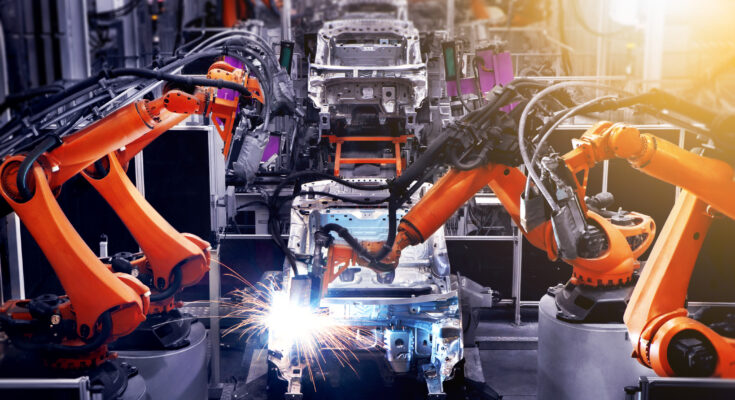
\includegraphics[height=6cm,width=10cm]{./Images/CH1/industrial_robot.jpg}
  	\caption{نمونه ربات صنعتی}
  	\label{ربات سنعتی}
    \end{figure}

\textbf{2- ربات‌های خدماتی}:
  ربات‌های خدماتی، نوعی سیستم هوش مصنوعی، به عنوان یک پیشرفت فناوری مهم در سال‌های اخیر ظهور کرده‌اند. این ربات‌ها برای انجام وظایف و عملکردهای متنوع در محیط‌های مختلف طراحی و برنامه‌ریزی شده‌اند تا زندگی انسان‌ها را بهبود بخشند و خدمات گوناگونی را فراهم آورند. برخلاف ربات‌های صنعتی که عمدتاً در کارخانه‌ها عمل می‌کنند، ربات‌های خدماتی برای تعامل مستقیم با انسان‌ها طراحی شده‌اند و در محیط‌های مختلفی نظیر خانه‌ها، مراکز درمانی، بخش هتل‌ها، فضاهای عمومی و غیره عمل می‌کنند.
\newpage
\begin{itemize}
	\item ربات‌های خانگی: این ربات‌ها در کمک به کارهای خانگی نظیر جارو‌کردن، کوتاه کردن چمن و تمیز کردن استفاده می‌شوند.
    \begin{figure}[!h]
	\vspace{0.2cm}
	\centering
	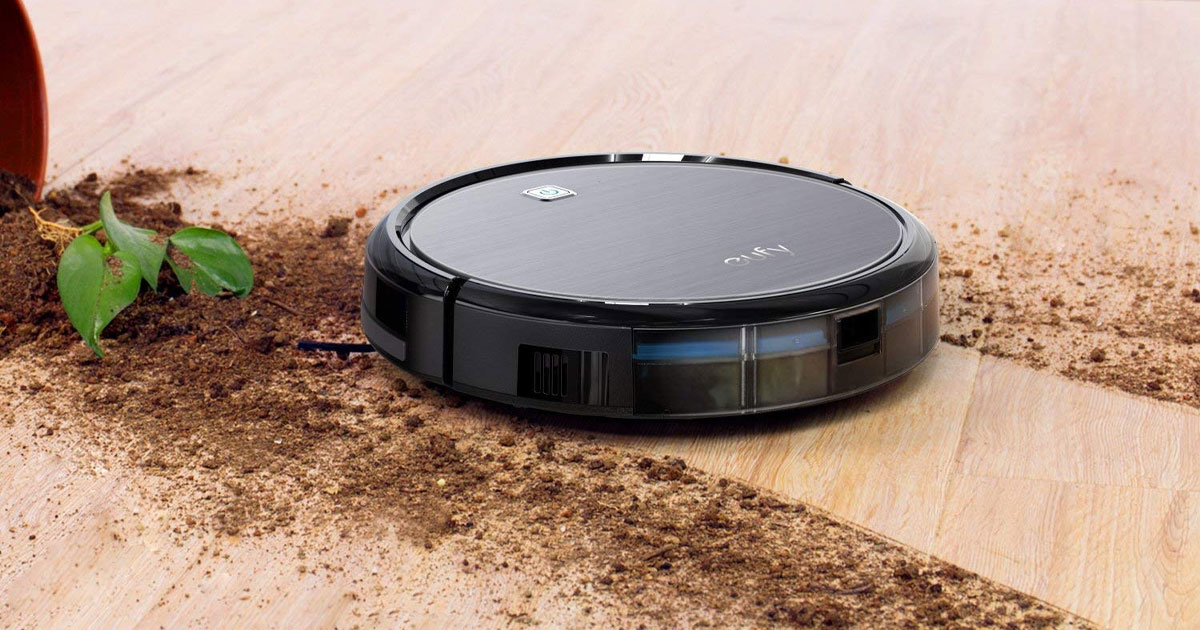
\includegraphics[height=4cm,width=7cm]{./Images/CH1/service_robot_2.jpg}
	\caption{نمونه‌ای از ربات خانگی}
	\label{ربات خانگی}
	\end{figure}
	
	\item ربات‌های پزشکی: در محیط‌های درمانی برای انجام عملیات‌های جراحی، مراقبت از بیماران و بازسازی استفاده می‌شوند.
    \begin{figure}[!h]
	\vspace{0.2cm}
	\centering
	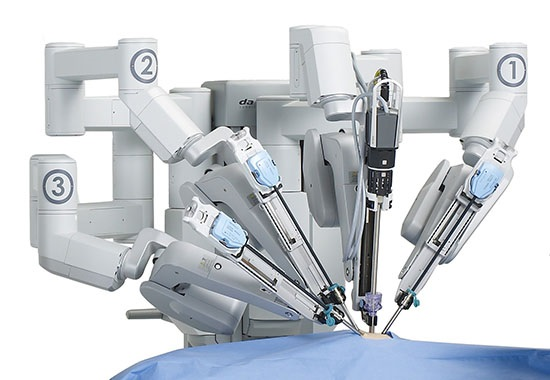
\includegraphics[height=4cm,width=7cm]{./Images/CH1/service_robot_3.jpg}
	\caption{ربات جراح}
	\label{ربات جراح}
	\end{figure}

	\item ربات‌های سرگرمی: برای اهداف سرگرمی طراحی شده‌اند، از اسباب‌بازی‌ها و همراهان رباتی تا کاربردهای سرگرمی دیگر.
	
    \begin{figure}[!h]
	\vspace{0.2cm}
	\centering
	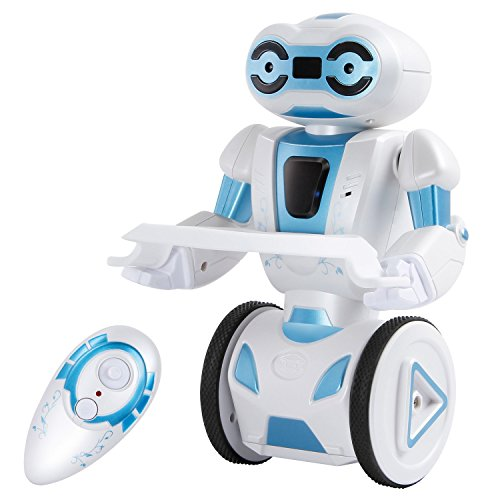
\includegraphics[height=4.5cm,width=7cm]{./Images/CH1/entertainment_robot1.jpg}
	\caption{یک نمونه ربات سرگرمی}
	\label{ربات سرگرمی}
	\end{figure}

\end{itemize}	
 
\textbf{3- وسایل خودران}:
  ربات‌های خودران می‌توانند وظایف خود را به‌صورت کاملاً خودکار و بدون نیاز به نظارت و کنترل انسان انجام دهند. این ربات‌ها معمولاً برای فعالیت در محیط‌های باز که فعالیت کردن در آن‌ها نیازی به نظارت انسان ندارد، طراحی شده‌اند. چنین ربات‌هایی طراحی منحصربه‌فردی دارند؛ زیرا با برخورداری از سنسورهای مختلف می‌توانند محیط اطراف خود را به‌خوبی درک کنند و سپس با بهره‌مندی با آن دسته از تجهیزات خود که برای تصمیم‌گیری به ربات کمک می‌کنند (معمولاً کامپیوترهای خاصی این کار را انجام می‌دهند)، بر اساس داده‌های در اختیار خود و همچنین مأموریتی که به آن‌ها محول شده است، تصمیم مناسب را برای انجام کار بعدی به بهترین شکل ممکن می‌گیرند.
    \begin{figure}[!h]
	\vspace{0.2cm}
	\centering
	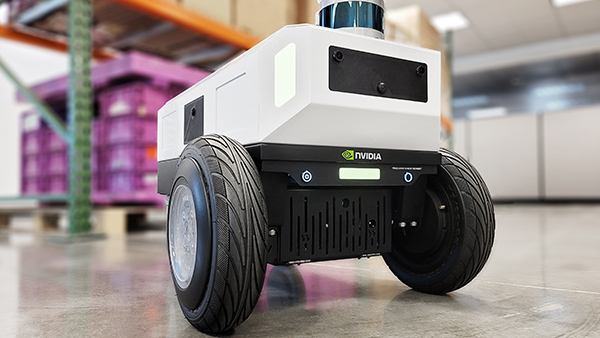
\includegraphics[height=4.7cm,width=8cm]{./Images/CH1/autonomous_robot.jpg}
‌	\caption{نمونه‌ای از ربات خودران}
	\label{ربات خودران}
	\end{figure}
	
\textbf{4- ربات‌های نظامی و دفاعی}:
  این ربات‌ها برای کاربردهای نظامی طراحی شده‌اند، از جمله نظارت، انجام مأموریت‌های مهم و مبارزه از راه دور. آنها در محیط‌های چالشی عمل می‌کنند تا خطرات برای سربازان انسانی را کمینه کنند.
  سلاح‌ها و تجهیزات نظامی رباتیک مجهز به هوش مصنوعی نیز می‌توانند یک برگ برنده طلایی برای پیروزی در جنگ‌ها باشند؛ به‌عنوان ‌مثال سامانه پیشرفته نظامی مدولار مارس
\lr{MAARS}
\unskip\LTRfootnote{Modular Advanced Armed Robotic System} 
با ظاهری شبیه به تانک مجهز به قابلیت پرتاب گاز اشک‌آور و انتشار اشعه لیزر جهت سردرگم کردن دشمن و همچنین یک نارنجک‌انداز برای زمین‌گیر کردن دشمن است\cite{Digiato}.
    \begin{figure}[!h]
	\vspace{0.2cm}
	\centering
	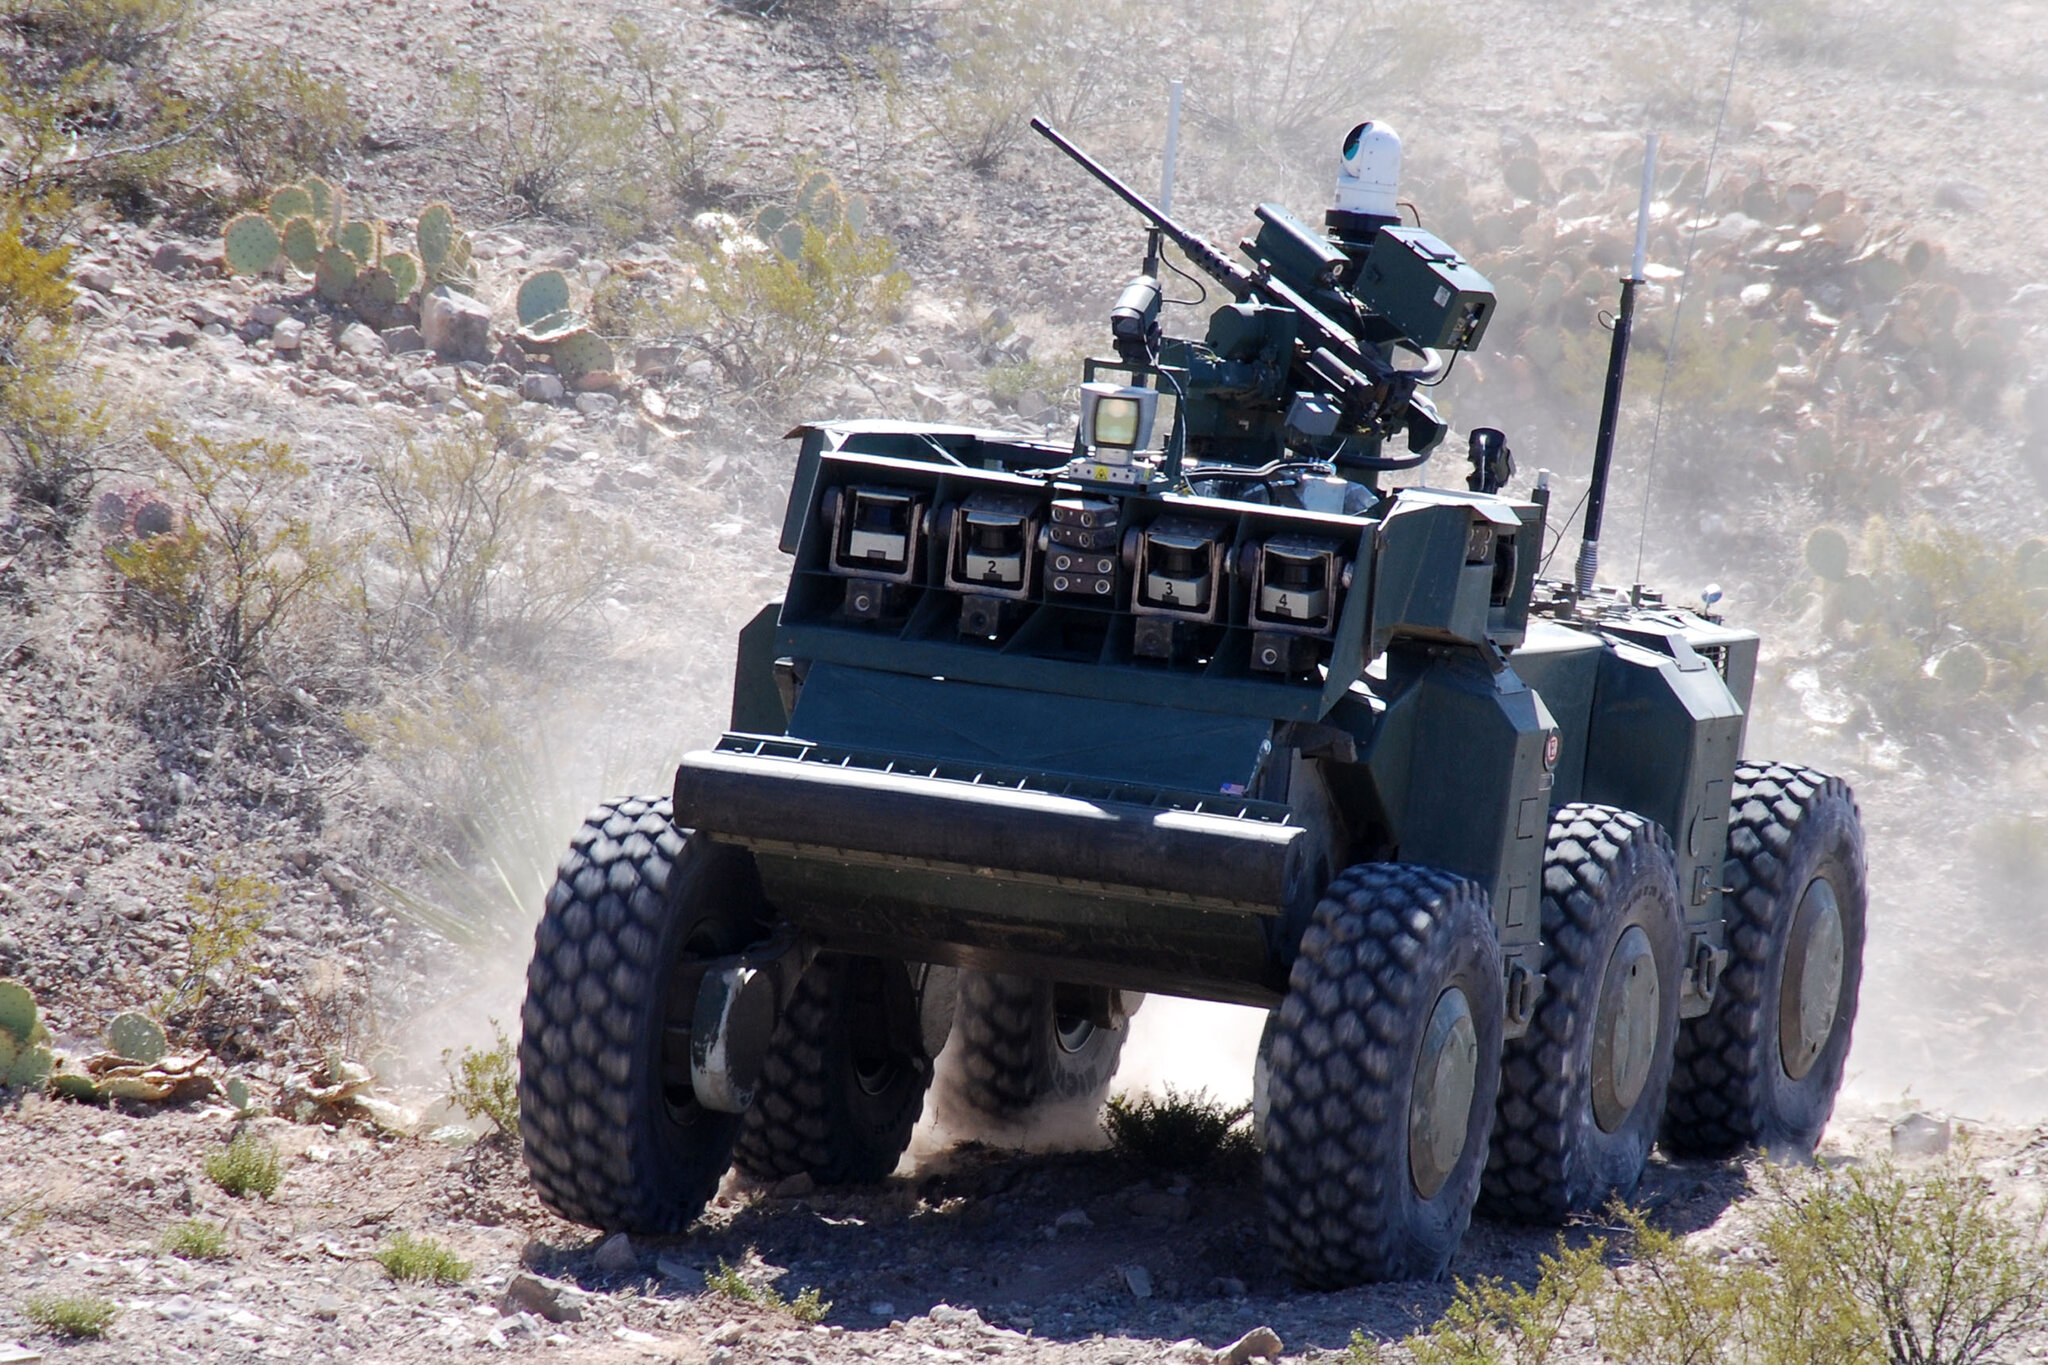
\includegraphics[height=4.7cm,width=8cm]{./Images/CH1/military_robot.jpg}
	‌\caption{ربات نظامی}
	\label{ربات نظامی}
	\end{figure}
\newpage
\textbf{5- ربات‌های آموزشی}:	
  ربات‌های آموزشی برای آموزش برنامه‌نویسی، مهندسی و مهارت‌های حل مسئله به دانش‌آموزان استفاده می‌شوند. آنها از کیت‌های ساده برای مبتدیان تا پلتفرم‌های پیچیده‌تر برای دانشجویان پیشرفته متفاوتی دارند.
    \begin{figure}[!h]
	\vspace{0.2cm}
	\centering
	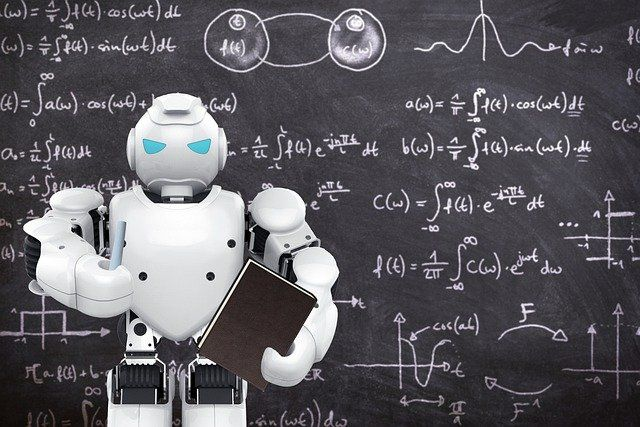
\includegraphics[height=6cm,width=10cm]{./Images/CH1/educational_robot.jpg}
	‌\caption{ربات آموزگار}
	\end{figure}
	
\textbf{6- ربات‌های کشاورزی}: 
  انجام برخی از امور کشاورزی توسط کشاورزان وقت زیادی از آن‌ها می‌گیرد. چنانچه آن‌ها برای انجام چنین کارهایی از ربات‌ها کمک بگیرند، شاهد نتیجه بهتری خواهند بود. این امور شامل فعالیت‌های مرتبط با کاشت و بذرپاشی، کنترل علف‌های هرز، برداشت و سایر فعالیت‌های مشابه می‌شود.
  
  برداشت محصولات کشاورزی با کمک ربات‌ها در مقایسه با انجام این کار به‌صورت سنتی و توسط کشاورزان، نیز نتیجه بهتری دارد. برای انجام این کار نیز ربات‌های مخصوصی طراحی شده‌اند. برخی از این ربات‌ها دارای بازوهای مخصوص برای برداشت و چیدن میوه‌های تابستانی حساس با بافت نرم مثل انگور، انواع توت‌ها و... جهت جلوگیری از آسیب دیدن آن‌ها هستند.
    \begin{figure}[!h]
	\vspace{0.2cm}
	\centering
	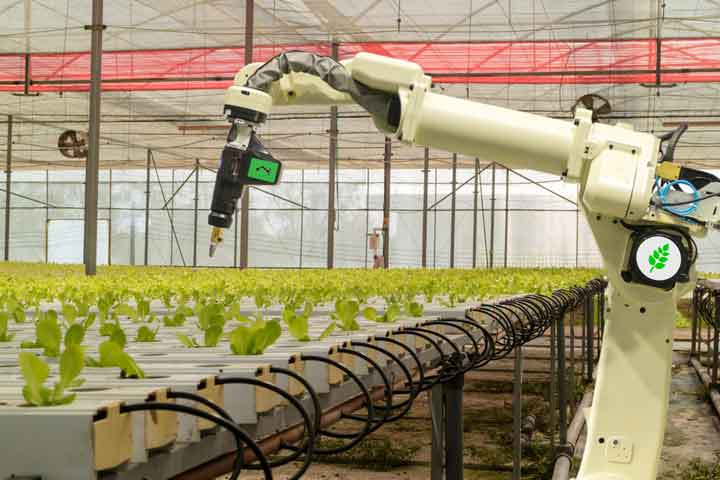
\includegraphics[height=6cm,width=10cm]{./Images/CH1/agricultural_robot.jpeg}
	‌\caption{یک نمونه ربات کشاورز}
	\label{ربات کشاورزی}
	\end{figure}
	
\textbf{7- ربات‌های پزشکی}: 
  ربات‌ها در این حوزه می‌توانند به‌عنوان دستیار جراح استفاده شوند. آن‌ها می‌توانند در جراحی قسمت‌های حساس بدن مثل گردن و ستون فقرات که کوچک‌ترین اشتباه در جراحی آن‌ها آسیب‌های جبران‌ناپذیری را به بار می‌آورد، کمک دست جراحان شوند و دقت جراحی را افزایش دهند. حتی برخی از جراحی‌ها به‌قدری دقت بالایی می‌طلبند که انسان قادر به انجام آن‌ها نیست و برای انجام آن‌ها ناگزیر باید از ربات استفاده کند؛ به‌عنوان مثال شرکت نورالینک
\unskip\LTRfootnote{Neuralink}
 قصد دارد یک تراشه مغزی برای برقراری ارتباط بین مغز انسان و دستگاه‌های مختلف جهت کنترل ذهن‌ها و همچنین درمان اختلالات و بیماری‌های مغزی عرضه کند و جراحی لازم برای قرار دادن این تراشه مغزی به‌قدری دقت زیادی می‌طلبد که انسان قادر به انجام آن نیست و نورالینک یک ربات برای این جراحی نیز طراحی کرده‌است.
    \begin{figure}[!h]
	\vspace{0.2cm}
	\centering
	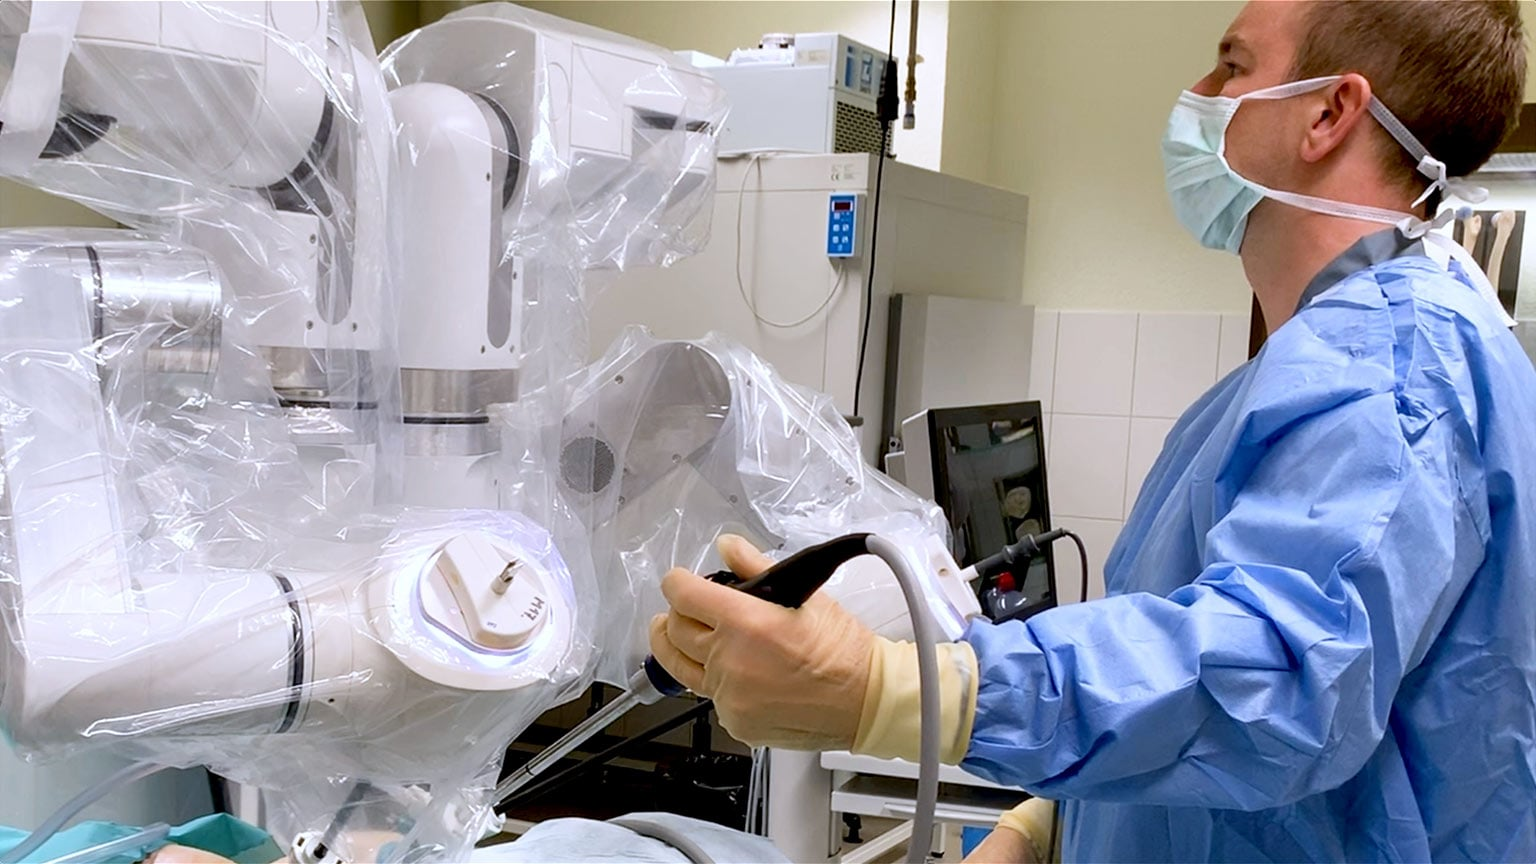
\includegraphics[height=4.6cm,width=8cm]{./Images/CH1/medical_robot.jpg}
	‌\caption{یک نمونه ربات پزشکی}
	\label{ربات پزشکی}
	\end{figure}
	
\textbf{8- ربات‌های انسان‌نما}:  
  ربات‌های انسان‌نما ظاهری شبیه به انسان دارند کارهای و رفتارهای او را تقلید می‌کنند. این ربات‌ها قادر به انجام فعالیت‌های شبیه به فعالیت‌های انسانی هستند که از میان آن‌ها می‌توان به دویدن، پریدن و حمل اشیا اشاره کرد. ظاهر برخی از ربات‌های انسان‌نما کاملاً شبیه انسان‌های واقعی است و اگر به‌صورت گذرا به آن‌ها نگاه کنیم یا از دور آن‌ها را ببینیم، اصلاً متوجه این موضوع نمی‌شویم.
    \begin{figure}[!h]
  	\vspace{0.2cm}
  	\centering
  	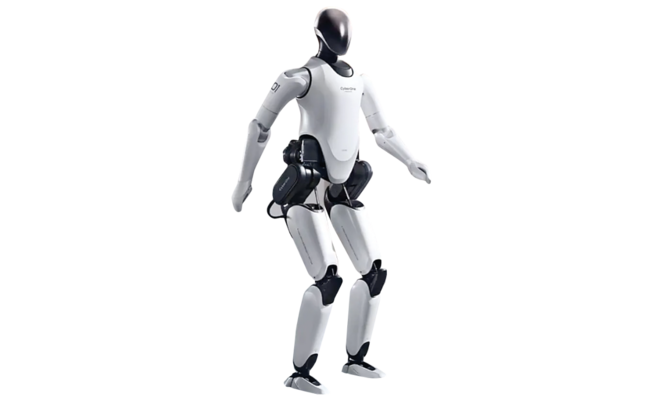
\includegraphics[height=4.6cm,width=8cm]{./Images/CH1/humanoid_robot.png}
  	‌\caption{ربات انسان‌نما}
  	\label{ربات انسان‌نما}
    \end{figure}
    
\section{ربات چهارپا}
در دنیای رباتیک، انواع مختلفی از ربات‌ها وجود دارند که با توجه به تنوع ویژگی‌هایشان، برای انجام وظایف گوناگون طراحی و ساخته می‌شوند. یکی از این انواع ربات‌ها که در سال‌های اخیر توجه زیادی به خود جلب کرده است، ربات‌های چهارپا (ربات‌های با چهار پا) هستند. این ربات‌ها با تقلید از حرکات و رفتار حیوانات دارای چهار پا مانند سگ، گربه و حتی عنکبوت‌ها طراحی می‌شوند.
\subsection{ویژگی‌های ربات چهارپا}
تمایل انسان به به‌كارگیري ظرفیت‌هاي طبیعت، بدست آوردن فهم بهتر از راه رفتن و حرکات چابک جانوران طبیعی، و الگوبرداري و شبیه‌سازي ماشینی رفتار حیوانات از جمله دلایل رویكرد به ربات‌هاي پادار است. در میان ربات‌هاي پادار، ربات‌هاي چهارپا به علت پایداري مناسب‌تر نسبت به ربات‌هاي دو پا و نیز تعداد پاهاي کمتر نسبت به ربات‌هاي شش پا، پیچیدگی کمتر را در طراحی داشته و مانورهاي مختلف ممكن را که از ربات‌هاي پادار انتظار می‌رود دارا است.

ربات‌هاي چهارپا نسبت به ربات‌هاي چرخ‌دار و شنی‌دار داراي مزایایی هستند که استفاده از آنها را در برخی زمینه‌ها توجیه می‌کند. از جمله این قابلیت‌ها می‌توان از سازگاري با محیط‌هاي ناهموار، جابجایی کارآمد، تعلیق پویاو فعال با زاویه دادن به بندگاه‌ها
\unskip\LTRfootnote{Joints}
،عبور از موانع، مصرف یكسان انرژي در محیط‌هاي هموار و ناهموار، امكان کاهش سر خوردگی با تماس عمودي با زمین نام برد.

با وجود مزایاي ذکر شده، ربات‌هاي پادار راه‌حل کامل مسئله حرکت نیست و مشكلات آنها باعث شده تا به‌كارگیري آنها در صنایع و بخش‌هاي خدماتی با کندي صورت گیرد. از جمله این مشكلات پیچیدگی، توان مصرفی بالا در مقایسه با ربات‌هاي چرخ‌دار در محیط‌هاي هموار، و سرعت کم آنها است.

\subsection{موارد کاربرد ربات‌های چهارپا}
موارد کاربرد ربات‌هاي چهارپا به مزیت‌هاي آنان نسبت به ربات‌هاي چرخ‌دار باز می‌گردد که شامل کمک به جمع‌آوري اطلاعات در امداد و نجات شهري به هنگام زلزله، آتش‌سوزي، و یا حوادث تروریستی و در جاهایی که حضور پرسنل انسانی داراي ریسک می‌باشد با امكان بالا رفتن و عبور از سطوح ناهموار، حمل بار از نقاط صعب العبور با کنترل از راه دور، اکتشافات سطحی و جستجو در کف دریاها، سطوح کرات
دیگر، قابلیت استفاده در محیط‌هاي پرمانع مانند محیط‌هاي جنگلی،کمک به افراد معلول در حرکت در محیط‌هاي ناهموار و نیز به عنوان ربات‌هاي توان‌بخشی می‌باشد\cite{Quadruped}.
\newpage
\subsection{نمونه‌های پیشین}
\begin{itemize}
\item  
\textbf{ربات آیبو}\unskip\LTRfootnote{AIBO}:
آیبو یک ربات کوچک چهارپا به شكل سگ است که در شرکت سونی
ساخته شده است. پروژه آیبو از سال 1990 شروع شده و مدل‌هاي
مختلفی از آن ساخته شد. مدلی از این ربات که در شکل
\ref{ربات آیبو}
مشاهده می‌شود در سال 2003 به منظور مسابقات جهانی ارائه گردید. این ربات به ازاي هرپا داراي سه درجه آزادي است و با هدف سرگرمی ساخته شده است که در طراحی این ربات از سرو موتورهاي جدیدي با گشتاور بالا استفاده شده است. این ربات براي یک ساعت حداقل بدون شارژ کردن مجدد می‌تواند کار کند\cite{AIBO}.
    \begin{figure}[!h]
	\vspace{0.2cm}
	\centering
	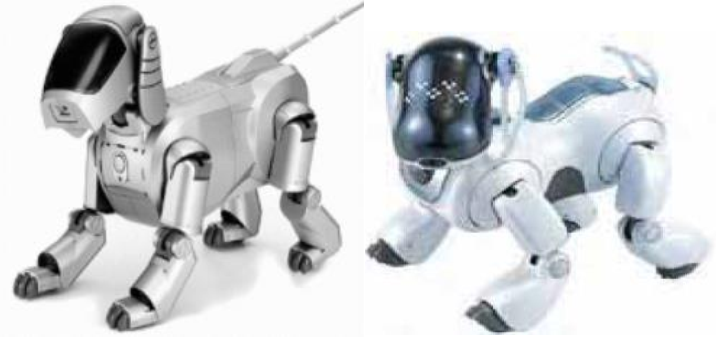
\includegraphics[height=4.5cm,width=7cm]{./Images/CH1/AIBO.png}
	‌\caption[ربات چهارپای آیبو]{ربات چهارپای آیبو\cite{AIBO}}
	\label{ربات آیبو}
	\end{figure}
	
\item	
\textbf{ربات جی-داگ}\LTRfootnote{G-Dog}:
کمپانی رباتیكی ژاپنی
\lr{HPI} 
 در حال تبلیغ جدیدترین محصول
تجاري خود به نام جی-داگ 3 با قیمتی معادل 550 یورو می‌باشد که در شكل
\ref{ربات جی‌داگ}
مشاهده می‌شود. واحد پردازشگر این ربات از نوع 
\lr{11-RPU}
است و ارتفاع ربات به 19 سانتیمتر می‌رسد. از طریق درگاه
\lr{RS232}
می‌توان اتصال میان ربات و کامپوتر برقرار و حرکات آن را برنامه‌ریزي نمود. این ربات داراي نه سرو موتور است که در هر پا دو موتور قرار گرفته‌است که در کل نه درجه آزادي به این ربات می‌دهد. قابلیت اضافه‌کردن موتورهاي اضافه نیز به این ربات وجود دارد\cite{G-Dog}.
    \begin{figure}[!h]	
	\vspace{0.2cm}
	\centering
	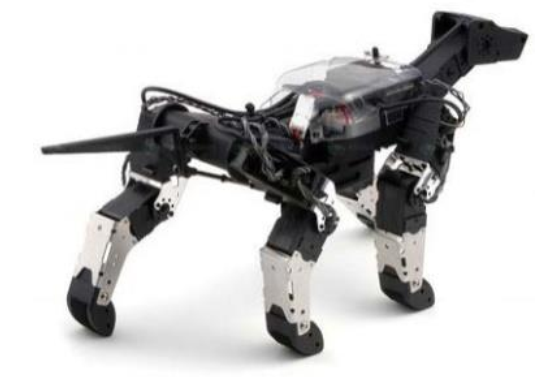
\includegraphics[height=4cm,width=6cm]{./Images/CH1/G_dog.png}
	‌\caption[ربات جی‌داگ]{ربات جی‌داگ\cite{G-Dog}}
	\label{ربات جی‌داگ}
	\end{figure}

\newpage
\item
\textbf{سگ کوچک}\unskip\LTRfootnote{Little Dog}:
سگ کوچک یک ربات چهارپاست که به منظور انجام تحقیقات در خصوص یادگیري گام‌برداري
\unskip\LTRfootnote{Locomotion}
به خصوص در زمین‌هاي ناهموار توسط شرکت بوستون داینمیكس در سال 2006 میلادي با حمایت
\lr{DARPA}\unskip\LTRfootnote{Defense Advanced Research Projects Agency}
ساخته شده\cite{Little-Dog-1} که در شكل
\ref{ربات سگ کوچک}
نمایش داده شده است. ربات سگ کوچک داراي  30 سانتیمتر طول، 18 سانتیمتر عرض، و 26 سانتیمتر ارتفاع است و وزن آن تقریباً برابر با 2/5 کیلوگرم است\cite{Little-Dog-2}.
این ربات داراي سه موتور الكتریكی براي کنترل هر پا می‌باشد که
مجموعا 12 درجه آزادي را به آن می‌دهند. در طراحی این ربات سعی
شده که موتورها تا حد امكان در نزدیكی بدن قرار گرفته تا اندازه پاها کوچک بمانند. همچنین از یک فنر براي گرفتن ارتعاشات سطوح در
پایین هر پا استفاده شده است. هر کدام از راه‌اندازنده موتورها با فرکانس 100هرتز با یک کنترلگر
\lr{PD} 
زاویه و یا گشتاور توسط یک کامپیوتر تحت سیستم عامل
\lr{Linux}
کنترل میگردد. سگ کوچک داراي چهار حسگر تماس در پاها و یک حسگر مجاورتی
\unskip\LTRfootnote{Proximity}
در سر و حسگر زاویه در تمامی بندگاه ها، و یک واحد اندازه‌گیري اینرسی
\lr{(IMU)}\unskip\LTRfootnote{Inertial Measuring Unit}
براي تنظیم موقعیت بدنه و شتاب آن است. سگ کوچک داراي یک باتري قابل شارژ است که انرژي آن را براي 30 دقیقه حرکت مستمر تأمین می‌نماید\cite{Little-Dog-2}.
    \begin{figure}[!h]
	\vspace{0.2cm}
	\centering
	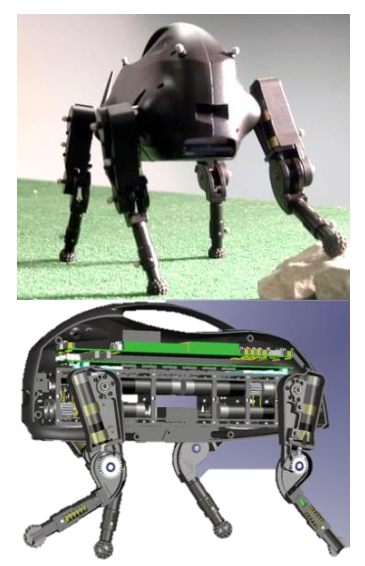
\includegraphics[height=8cm,width=6cm]{./Images/CH1/small_dog.png}
	‌\caption[ربات سگ کوچک]{ربات سگ کوچک\cite{Little-Dog-1}}
	\label{ربات سگ کوچک}
	\end{figure}

\newpage
\item 
\textbf{سگ بزرگ}\unskip\LTRfootnote{Big Dog}:
ربات سگ بزرگ محصول شرکت بوستون داینامیكس
\unskip\LTRfootnote{Boston Dynamics}
است و داراي قابلیت‌هاي منحصر به فردي در مانور دادن در محیط‌هاي طبیعی و خشن می‌باشد. این ربات قادر است بارهاي نسبتا سنگین تا حدود دو برابر وزن خود را در زمین‌هاي شیب دار، برفی و یخ زده حمل نماید. ربات سگ بزرگ قادر به دویدن می‌باشد و در حال حاضر به عنوان پیشرفته‌ترین ربات چهارپا در جهان شناخته می‌شود. ساخت این ربات تحت حمایت 30 میلیون دلاريِ آژانس طرح‌هاي پژوهشی پیشرفته دفاعی
\lr{DARPA} 
انجام گردیده است و در افغانستان نیز عملیات آزمایشی انجام داده است. 

ربات سگ بزرگ 109 کیلوگرم وزن دارد و 1 متر ارتفاع، 1/1 متر طول و 0/3 متر عرض دارد. این ربات قادر است 50 کیلوگرم بار را حمل نماید و نیز قادر است بدون بار مسافت 10 کیلومتر را در 2/5 ساعت بدون سوخت‌گیري طی نماید. این چهارپا قادر به پرش تا 1/1 متر نیز می‌باشد.
همان‌گونه که در شكل 1-14 مشاهده می‌شود، هر پاي این ربات داراي 4 درجه آزادي فعال (دو عدد در لگن، و یكی در زانو و یكی در مچ) و یک درجه آزادي غیر فعال (در فنر مچ پا) است. نیروي محرکه آن توسط یک موتور بنزینی تک سیلندر 15 اسب بخار و سیستم هیدرولیک با فشار
\lr{psi} 3000 
 تأمین می‌شود. هر پا توسط چهار شیر سرو الكتروهیدرولیک دو مرحله‌اي کنترل می‌گردد\cite{Big-Dog}.
    \begin{figure}[!h]
	\vspace{0.2cm}
	\centering
	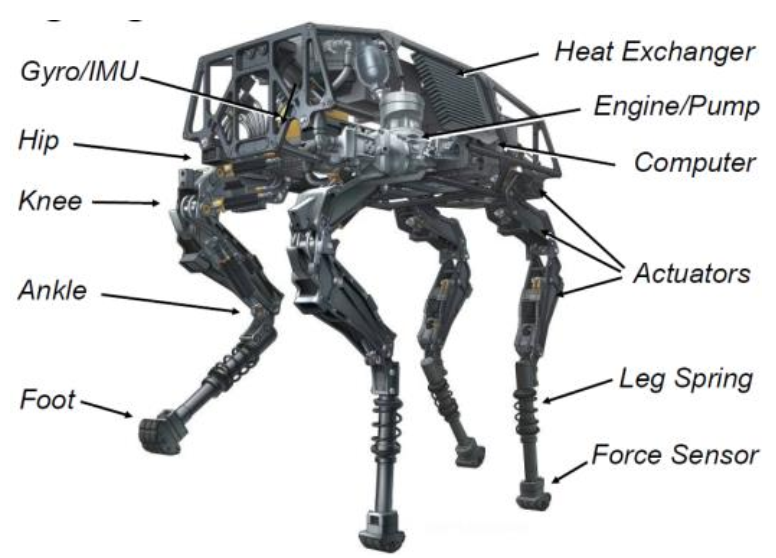
\includegraphics[height=9cm,width=13cm]{./Images/CH1/big_dog.png}
	‌\caption[ربات سگ بزرگ]{ربات سگ بزرگ\cite{Big-Dog}}
	\label{ربات سگ بزرگ}
	\end{figure}

\newpage
سگ بزرگ داري حسگرهاي متعددي است که شامل: 16 پتانسیومتر خطی براي اندازه‌گیري تغییر زوایاي بندگاه‌هاي زانو، لگن، و مچ پا، 16 عدد حسگر بار 
\unskip\LTRfootnote{Load cell}
براي پاها، 16 عدد حسگر جریان براي پایش جریان شیرهاي سرو، 3 عدد دوربین براي بینایی سه بعدي، یک عدد رادار لیزري (لیدار)
\unskip\LTRfootnote{Lidar}
،یک عدد ژایروسکوپ 
\unskip\LTRfootnote{Gyroscope}
که تغییرات سه زاویه و شتاب خطی سه محور را می‌دهد، دو عدد حسگر ولتاژ باتري می‌باشد. شكل
\ref{حسگر ربات سگ بزرگ}
محل قرار گیري حسگرها را در سگ بزرگ نشان می‌دهد.
    \begin{figure}[!h]
	\vspace{0.2cm}
	\centering
	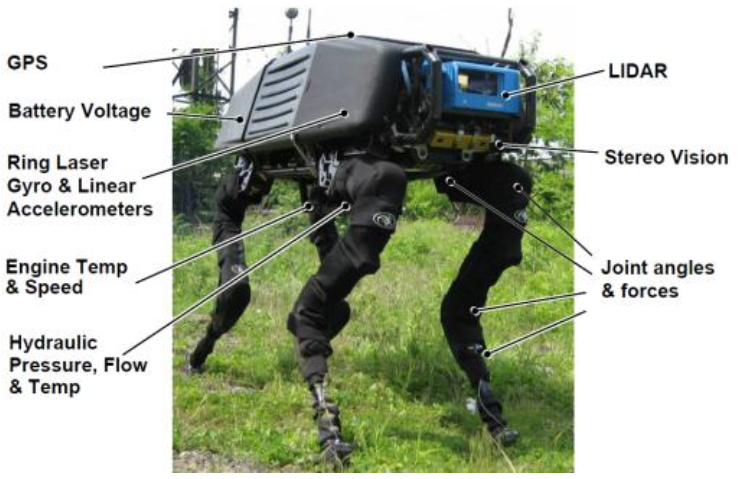
\includegraphics[height=6cm,width=12cm]{./Images/CH1/big_dog_sensors.png}
	‌\caption{حسگرهاي ربات سگ بزرگ و محل قرارگیري آنها}
	\label{حسگر ربات سگ بزرگ}
	\end{figure}

کامپیوتر روي ربات به‌صورت سفارشی تهیه شده است و داراي پردازشگر پنتیوم با سیستم عامل بلادرنگ
\lr{QNX}
 می‌باشد. کد برنامه به زبان
\lr{C++}
 نوشته شده‌است که اطلاعات حسگرها را دریافت و کنترل لازم به راه‌اندازها را اعمال می‌کند و نیز ارتباط با کاربر را نیز فراهم می‌نماید. معماري نرم افزار ربات سگ بزرگ در شكل
\ref{معماری سگ بزرگ}
نمایش داده شده است.
    \begin{figure}[!h]
 	\vspace{0.2cm}
 	\centering
 	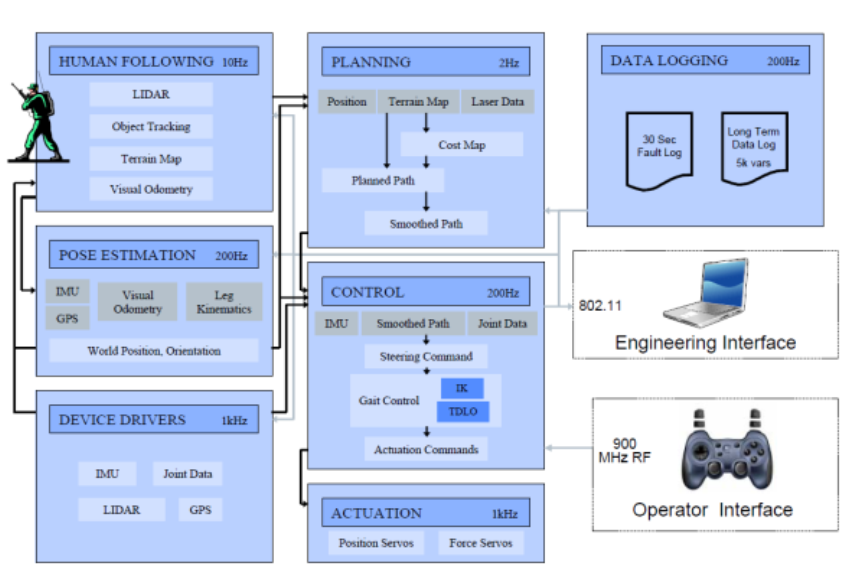
\includegraphics[height=5.5cm,width=13cm]{./Images/CH1/big_dog_structure.png}
 	‌\caption{معماري نرم‌افزار ربات سگ بزرگ}
 	\label{معماری سگ بزرگ}
 	\end{figure}
 
فرکانس نمونه‌برداري براي اطلاعات مربوط به مسیریابی 2 هرتز، فاصله‌یابی و تشخیص موانع 10 هرتز، تخمین موقعیّت، کنترل و ثبت داده 200 هرتز، محرّک‌ها و راه‌اندازها یک کیلوهرتز می‌باشد. همچنین جلیقه‌اي براي کاربر ربات طراحی گردیده است که با تجهیزات نصب شده بر روي آن کاربر می‌تواند از طریق یک ارتباط رادیویی بی‌سیم 900 مگاهرتز اطلاعات دریافت شده توسط ربات را پایش کرده، و از طریق یک اهرم کنترل، حرکت ربات را کنترل کند.

نمونه پیشرفته تر ربات سگ بزرگ به‌ نام سامانه پشتیبان گروهان
\lr{(LS3)}
\unskip\LTRfootnote{Legged Squad Support System}
 یا سگ آلفا و نیز گربه وحشی
\unskip\LTRfootnote{WildCat}
 می‌باشد که اخیراً توسط همین شرکت و تحت حمایت وزارت دفاع آمریكا ساخته شده است که در شكل
\ref{ربات پشتیبان گروه}
و
\ref{گربه وحشی}
قابل مشاهده‌اند\cite{LS3}\cite{Wild-Cat}. این ربات‌ها بیشتر جنبه نمایشی نظامی داشته و هنوز اطلاعات مستندي در مورد آنها در مقالات علمی موجود نیست. گربه وحشی نمونه پیشرفته تر ربات یوزپلنگ
\lr{MIT}
است و هم اکنون مراحل آزمون و اصلاحات خود را طی می‌کند و قرار است تا سرعت   50 کیلومتر در ساعت بدود.
    \begin{figure}[!h]
	\vspace{0.2cm}
	\centering
	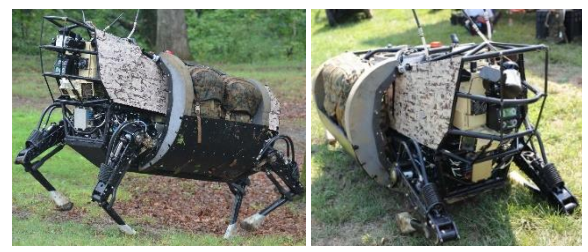
\includegraphics[height=5cm,width=13cm]{./Images/CH1/LS3_robot.png}
	‌\caption[دو تصویر از ربات سامانه پشتیبان گروه]{دو تصویر از ربات سامانه پشتیبان گروه\cite{LS3}}
	\label{ربات پشتیبان گروه}
	\end{figure}

    \begin{figure}[!h]
	\centering
	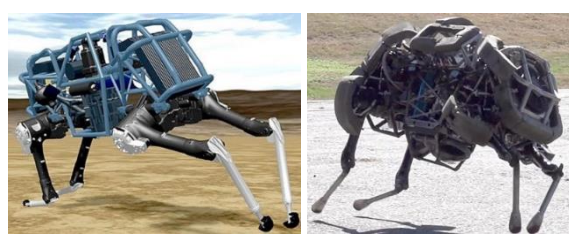
\includegraphics[height=5cm,width=13cm]{./Images/CH1/wild_cat_robot.png}
	‌\caption[گربه وحشی]{گربه وحشی\cite{Wild-Cat}}
	\label{گربه وحشی}
	\end{figure}
	
\newpage	
\item
\textbf{چهارپاي پیرو}:
ربات پیرو
\unskip\LTRfootnote{PQ1-PIRO}
که به طول 50 سانتیمتر می‌باشد، محصول انستیتو کره‌اي پوهانگ 
\unskip\LTRfootnote{Pohang Institute of Intelligent Robotics}
است. ربات چهارپاي پیرو براي انجام عملیاتی نظیر جستجو، کشف و حمل بار در شرایط طبیعی در نظر گرفته شده است (شكل
\ref{ربات پیرو}).
از آنجا که این ربات شباهت زیادي به ربات سگ بزرگ دارد، بسیاري آن را نمونه کره‌اي سگ بزرگ قلمداد کرده و این امر را نشانه علاقه کره به رقابت در عرصه رباتیک در تراز نخست می‌دانند. این ربات داراي سه درجه آزادي در هر پا می‌باشد\cite{Piro}.
    \begin{figure}[!h]
	\centering
	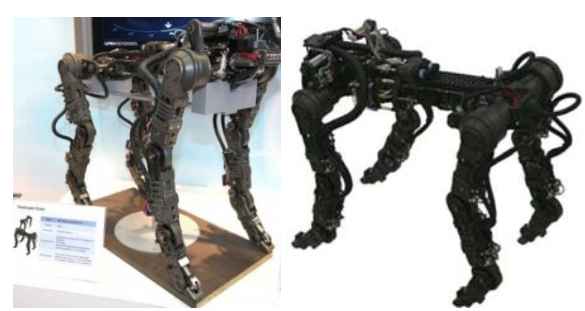
\includegraphics[height=4.4cm,width=12cm]{./Images/CH1/PIRO_robot.png}
	\caption[ربات چهارپاي پیرو]{ربات چهارپاي پیرو\cite{Piro}}
	\label{ربات پیرو}
	\end{figure}
	
\item
\textbf{ربات‌هاي آیدین}:
ربات آیدین 1و2و3 
\lr{(AiDIN)}\unskip\LTRfootnote{Artificial Digitigrade for Natural Environment}
ساخت آزمایشگاه رباتیک هوشمند وسیستم‌هاي مكاترونیک
\unskip\LTRfootnote{Intelligent Robotics and Mechatronic Systems Laboratory}
درکره شمالی در سال‌هاي 2007، 2008 و 2013 می‌باشد\cite{Aidin-I-2}\cite{Aidin-III-1}\cite{Aidin-III-2}\cite{Aidin-I-1}. شكل
\ref{ربات آیدین}
نمایی از این دو نسل ربات را نشان می‌دهد. این ربات داراي 10 درجه آزادي فعال و 4 درجه آزادي غیر فعال است. همانطور که در شكل مشاهده می‌شود، پاهاي جلو هرکدام داراي  3 درجه آزادي فعال و یک غیر فعال به صورت فنر و پاهاي عقب داراي 2 درجه آزادي فعال و یک غیر فعال به صورت فنر می‌باشد. پاهاي ربات آیدین2 داراي وزن کمتر و نسبت ساق به ران آن مناسب‌تر انتخاب شده است و نیز مكان مرکز ثقل پاها براي پایداري بهتر اصلاح گردیده است.
    \begin{figure}[!h]
	\centering
	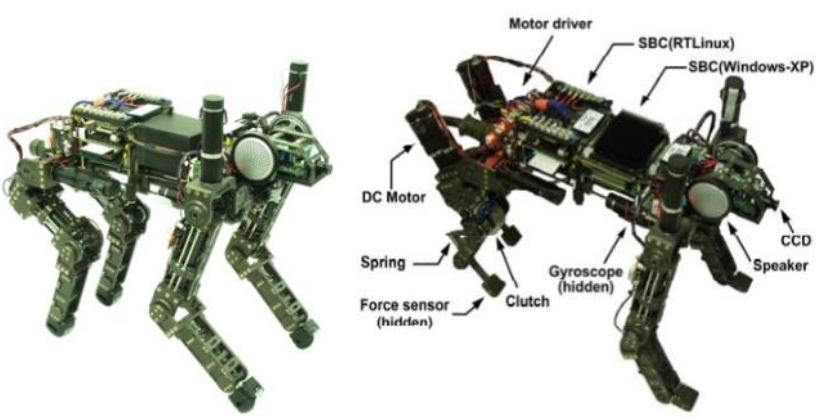
\includegraphics[height=4.4cm,width=12cm]{./Images/CH1/AiDIN_robot.png}
	\caption[نماي ربات آیدین ( 1راست) و آیدین ( 2چپ)]{نماي ربات آیدین ( 1راست) و آیدین ( 2چپ)\cite{Aidin-I-1}}
	\label{ربات آیدین}
	\end{figure}	

\newpage
هر بندگاه فعّال توسط یک موتور جریان ثابت 20 وات با جعبه با نسبت دور  53:1 تحریک می‌گردد. ربات آیدین داراي دو کنترل‌گر درونی
\unskip\LTRfootnote{Embeded Controller}
اصلی است که به‌صورت کامپیوترهاي تک بُرد پنتیم 3 با فرکانس 800 مگاهرتز با دیسک فلش و کنترل‌گر
\lr{CAN}
\unskip\LTRfootnote{Controller Area Network}
تحت سیستم عامل بلادرنگ
\lr{RTLinux} 
می‌باشد. کامپیوتر تک بورد دیگر که پنتیوم 1/1 گیگاهرتز و داراي شبكه بیسیم است، وظیفه پردازش صدا و تصویر را دارد. انرژي ربات توست یک سیم برق 220 ولت تأمین می‌گردد ولی تمام تبادل اطلاعات ربات با کاربر از طریق شبكه بی‌سیم انجام می‌پذیرد. این ربات همچنین داراي 10 کنترل‌گر کوچک از نوع
\lr{MicroChip PCI 18f458}
می‌باشد که هرکدام به‌طور محلّی یكی از درجات آزادي را کنترل می‌کند.

\item
\textbf{چهارپای هانما}:
چهارپاي هانما
\unskip\LTRfootnote{Hanma}
در سال 2010 در پژوهشكده رباتیک دانشگاه شاندانگ
\lr{(SUCRO)}
\unskip\LTRfootnote{Shandong University Center for Robotics}
چین ساخته شده که داراي 12 درجه آزادي و 50 کیلوگرم وزن بود که البته برق آن از خارج از ربات تأمین می‌گردد\cite{Hanma}. ارتفاع ربات در حالت اولیه 67 سانتی‌متر و طول و عرض آن به ترتیب  100و 40 سانتی‌متر است. براي حرکت بندگاه‌هاي ربات از محرک‌هاي هیدرولیكی استفاده شده است و قادر است 80 کیلوگرم بار را با سرعت  40 سانتی‌متر بر ثانیه منتقل نماید. شكل
\ref{ربات هانما}
دو نما از این ربات چهارپا را نشان می‌دهد.
    \begin{figure}[!h]
	\centering
	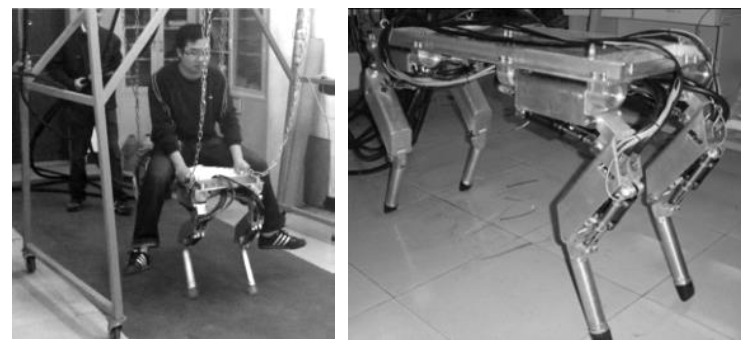
\includegraphics[height=6cm,width=10cm]{./Images/CH1/Hanma_robot.png}
	\caption[ربات چهارپاي هانما]{ربات چهارپاي هانما\cite{Hanma}}
	\label{ربات هانما}
	\end{figure}

\newpage	
\item
\textbf{چهارپاي هایكیو}:
ربات‌ هایكیو
\unskip\LTRfootnote{HyQ}
ساخت انستیتو تكنولوژي ایتالیاست که داراي 12 درجه آزادي است و موقعیت و گشتاور بندگاه‌هاي آن به‌وسیله بازوهاي هیدرولیكی کنترل می‌گردد\cite{HyQ}. وزن ربات حدود 75 کیلوگرم و داراي یک متر طول و نیم متر عرض است و جثه آن به اندازه یک بز می‌باشد.

سامانه کنترل این ربات بر روي یک کامپیوتر تک بورد
\lr{PC104}
تحت لینوکس زمان واقعی با پچ
\lr{Xenomai} 
 اجراء می‌گردد. این ربات می‌تواند علاوه بر قدم زدن، به‌صورت یورتمه نیز حرکت نماید. شكل
 \ref{ربات هایکیو}
 تصاویري از این ربات را نشان می‌دهد.
    \begin{figure}[!h]
	\centering
	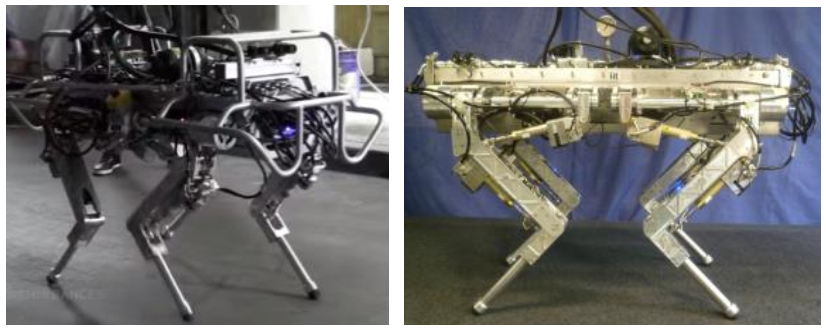
\includegraphics[height=5cm,width=10cm]{./Images/CH1/HyQ_robot.png}
	\caption[ربات چهارپاي هایكیو]{ربات چهارپاي هایكیو\cite{HyQ}}
	\label{ربات هایکیو}
	\end{figure}
	
\end{itemize}

\section{جمع بندی}
زمینه رباتیک شامل طیف گسترده‌ای از انواع ربات‌ها است، هر کدام برای کاربردها و وظایف خاصی طراحی شده‌اند. از محیط‌های صنعتی تا بهداشت، از کاوش‌ها تا آموزش، ربات‌ها پتانسیل تحول در صنایع را دارند و به شکل‌های مختلفی به زندگی‌های ما اضافه ارزش می‌دهند. با پیشرفت فناوری، انتظار داریم که نوآوری‌های بیشتری را ببینیم و انواع جدیدی از ربات‌ها با قابلیت‌های پیشرفته‌تر پدیدار شوند.
\newpage
\section{ساختار پایان‌نامه}
پایان‌نامه شامل 5 فصل است؛ در فصل اول، ربات و انواع آن با تاکید بر ربات‌های چهارپا، ویژگی‌ها، موارد کاربرد و نمونه‌های پیشین آورده شده است. در فصل دوم، به کمک نرم‌افزار سالیدورکس، قطعات ربات طراحی و ابعاد آن‌ها محاسبه شد. همچنین با بهبود نمونه اولیه سعی در رفع عیوب نموده تا به نمونه نهایی از ربات دست یافته شود. در فصل سوم، تمرکز بر سخت‌افزار ربات شده است و اجزائی مانند سرو موتور، میکروکنترلر، ماژول \lr{Arduino} و دوربین ربات مورد بررسی قرار گرفته است. در فصل بعدی، پروتکل \lr{UART}، تکنیک کنترلی \lr{PWM}، تنظیمات لازم میکروکنترلر در نرم‌افزارهای \lr{CubeMX} و \lr{Keil} انجام شد. در نهایت در فصل پنجم نتیجه‌گیري و پیشنهادات لازم آورده شده است.